\documentclass{article}
	
\usepackage[margin=1in]{geometry}		% For setting margins
\usepackage{amsmath}				% For Math
\usepackage[]{amssymb}
\usepackage{amsmath}
\usepackage{gensymb}
\usepackage{fancyhdr}				% For fancy header/footer
\usepackage{graphicx}				% For including figure/image
\usepackage{cancel}					% To use the slash to cancel out stuff in work
\usepackage{wasysym}                % For cent symbol
\usepackage{needspace}              % To force item to next page
\usepackage{mathtools}

%%%%%%%%%%%%%%%%%%%%%%
% Set up fancy header/footer
\pagestyle{fancy}
\fancyhead[RO,R]{{\large\textbf{PHYS-102}}}
\fancyhead[LO,L]{\large{\textbf{Ch 32 Problem Set}}}
% \fancyhead[CO,C]{\large{\textbf{Part 1}}}
% \fancyhead[RO,R]{\today}
\fancyfoot[LO,L]{}
\fancyfoot[CO,C]{\thepage}
\fancyfoot[RO,R]{}
\renewcommand{\headrulewidth}{0.4pt}
\renewcommand{\footrulewidth}{0.4pt}
%%%%%%%%%%%%%%%%%%%%%%

\newcommand{\hmwkTitle}{Chapter 32 Light: Reflection and Refraction}
% \newcommand{\hmwkDueDate}{February 12, 2014}
\newcommand{\hmwkClass}{PHYS-102}
% \newcommand{\hmwkClassTime}{}
% \newcommand{\hmwkClassInstructor}{Professor Isaac Newton}
\newcommand{\hmwkAuthorName}{\textbf{\underline{\hspace{3in}}}}

% math shortcuts
\newcommand\rr{\quad\Rightarrow\quad}
\newcommand{\spc}{\vspace{1em}\hrule\vspace{1em}}
\newcommand{\bp}[1]{\left(#1\right)}
\newcommand{\bb}[1]{\left[#1\right]}

%
% Title Page
%

\title{
    \vspace{2in}
    \textmd{\textbf{\hmwkTitle}}\\
    \vspace{0.5in}
    \textmd{\textbf{\hmwkClass}}\\
    % \normalsize\vspace{0.1in}\small{Due\ on\ \hmwkDueDate\ at 3:10pm}\\
    % \vspace{0.1in}\large{\textit{\hmwkClassInstructor\ \hmwkClassTime}}
    \vspace{4in}
}

\author{\hmwkAuthorName}
\date{}
\begin{document}
\maketitle
\newpage
\begin{center}
    \section*{\textbf{\underline {Conceptual Questions}}}
\end{center}
\subsubsection*{
    2. Archimedes is said to have burned the whole Roman fleet in the harbor
    of Syracuse by focusing the rays of the Sun with a huge spherical mirror.
    Is this reasonable?
}
Yes, having a huge spherical mirror, would result in many rays of the sun to be
at a focus point where the object it points at will absorb these rays (and
energy conversion to thermal energy)
\subsubsection*{
    3. What is the focal length of a plane mirror? What is the magnification
    of a plane mirror?
}
Since the mirror equation holds true for a plane mirror, the focal length is
$f=\frac r 2$ where $r=\infty$ since the radius of a flat surface is infinity. This
would result in the focal length also to be infinity. The magnification of a
plane mirror would be 1 since there is equal distance between object and image 
\subsubsection*{
    4. An object is placed along the principal axis of a spherical mirror.
    The magnification of the object is -3.0. Is the image real or virtual,
    inverted or upright? Is the mirror concave or convex? On which side of
    the mirror is the image located?
}
The image is real and inverted, because the magnification is negative. The
mirror is concave because convex can only form virtual images. The image is on
the same side of the mirror as the object; real images are formed by converging
light rays and light rays cannot actually pass through a mirror
\subsubsection*{
    7. If a concave mirror produces a real image, is the image necessarily
    inverted?
}
Yes. When a concave mirror produces a real image, both $d_0$ and $d_i$ are
positive which would indicate a negative magnification by the equation for
magnification $m=-\displaystyle\frac{d_i}{d_0}$. A negative magnification means the image is
inverted 
\subsubsection*{
    8. How might you determine the speed of light in a solid, rectangular,
    transparent object?
}
Rays entering the object will have an incident angle and a resulting angle of
refraction. Using Snell's law, we know one of the mediums is air, and we would
solve for the other medium, $n_2$, assuming, geometrically, we can find the
angle of the refracted ray with respect to the normal. We can then find the
speed of light in the object using the index of refraction and its relationship
with c in a vacuum given by $n = \displaystyle\frac{c}{v} \rr v =
\displaystyle\frac c n$
\begin{figure}[h]
    \begin{center}
        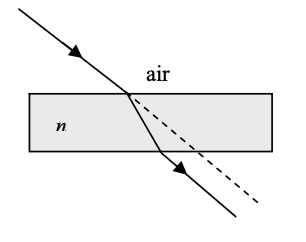
\includegraphics[width=0.3\textwidth]{figures/q8a.jpg}
    \end{center}
\end{figure}
\subsubsection*{
    11. What is the angle of refraction when a light ray is incident
    perpendicular to the boundary between two transparent materials?
}
The angle of refraction and angle of incidence are both zero in this case.
\subsubsection*{
    14. When a wide beam of parallel light enters water at an angle,
    the beam broadens. Explain.
}
Because the broad beam hits the surface of the water at an angle, it illuminates
an area of the surface that is wider than the beam width. Light form the beam
bends towards the normal. The refracted beam is wider than the incident beam
because one edge of the beam strikes the surface first, while the other edge
travels farther in the air. 
\begin{figure}[h]
    \begin{center}
        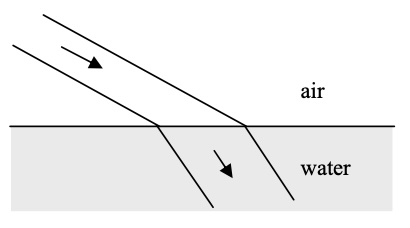
\includegraphics[width=0.3\textwidth]{figures/q14a.jpg}
    \end{center}
\end{figure}
\subsubsection*{
    17. A ray of light is refracted through three different materials.
    Rank the materials according to their index of refraction,
    least to greatest.
}
\begin{figure}[h]
    \begin{center}
        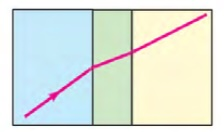
\includegraphics[width=0.3\textwidth]{figures/q17.jpg}
    \end{center}
\end{figure}
Let each section be 1, 2, 3 from left to right. From 1 to 2, the beam bends
towards the normal, which means that the index of refraction of 2 is greater
than 1. When 2 goes to 3, the beam bends away from normal but not enough to get
back to parallel with 1. So that means the index of refraction is less than 2,
but greater than 1. Therefore, from least to greatest would be: 1, 3, 2.
\subsubsection*{
    18. Can a light ray traveling in air be totally reflected when it
    strikes a smooth water surface if the incident angle is chosen
    correctly? Explain.
}
No. Total Internal Reflection can only occur if traveling from a medum of higher
index of refraction to lower.
\subsubsection*{
    20. What type of mirror is shown?
}
\begin{figure}[h]
    \begin{center}
        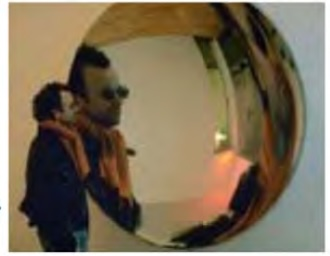
\includegraphics[width=0.3\textwidth]{figures/q20.jpg}
    \end{center}
\end{figure}
The mirror image is virtual and upright and the object is standing inside the
focal point with a seemingly positive magnification so, the mirror is concave.
A convex mirror woulds still result in a virtual, upright image, but it would be
smaller. 
\newpage
\begin{center}
    \section*{\textbf{\underline {Problems}}}
    \subsection*{\textbf{\textit{32-3 Spherical Mirrors}}}
\end{center}
\subsubsection*{
    9. A solar cooker, really a concave mirror pointed at the Sun,
    focuses the Sun’s rays 18.8 cm in front of the mirror. What is
    the radius of the spherical surface from which the mirror was made?
}
\begin{align*}
    \intertext{Since $r=\frac r 2$ and we are given $f$}
    r &= 2f = 2(18.8\;cm) \\
    \Aboxed{r &= 37.6\;cm}
\end{align*}
\subsubsection*{
    10. How far from a concave mirror (radius 24.0 cm) must an object be
    placed if its image is to be at infinity?
}
\begin{align*}
    \intertext{For an object to be at infinity, it must be at the focal point.}
    f &= \displaystyle\frac{r}{2} = \displaystyle\frac{24.0\;cm}{2} \\
    \Aboxed{f &= 12.0\;cm}
\end{align*}
\subsubsection*{
    13. You look at yourself in a shiny 9.2-cm-diameter Christmas tree ball.
    If your face is 25.0 cm away from the ball’s front surface, where is your
    image? Is it real or virtual? Is it upright or inverted?
}
\begin{align*}
    \intertext{Assuming a convex mirror (\textit{ball}), $d_0 = 25.0$ cm, $r =
    \frac 1 2 d = -4.6$ cm [convex mirror so radius is negative], $f=\frac r 2 =
-2.3$ cm}
\end{align*}
\intertext{Using the mirror equation,}
\begin{gather*}
    \displaystyle\frac{1}{d_0} + \displaystyle\frac{1}{d_i} =
    \displaystyle\frac{1}{f} \\
    \displaystyle\frac{1}{25.0\;cm}+\displaystyle\frac{1}{d_i} =
    \displaystyle\frac{1}{-2.3\;cm} \\
    \displaystyle\frac{1}{d_i} = -\displaystyle\frac{1}{2.3\;cm} -
    \displaystyle\frac{1}{25.0\;cm} \\
    d_i \approx -2.1\;cm
\end{gather*}
\intertext{If we find the magnification, we find that it is positive.}
\[
    m = -\displaystyle\frac{d_i}{d_0} \\
    m = -\displaystyle\frac{-2.1\;cm}{25.0\;cm} \approx +0.084 \\
\]
\Aboxed{\intertext{$\therefore$ we find that the image is virtual, upright and 2.1-cm behind the
surface of the Christmas tree ball.}}
\subsubsection*{
    16. Some rearview mirrors produce images of cars to your rear that are
    smaller than they would be if the mirror were flat. Are the mirrors
    concave or convex? What is a mirror’s radius of curvature if cars 18.0 m
    away appear 0.33 their normal size?
}
\intertext{Convex, and if $m=-\frac{d_i}{d_0}$,}
\begin{align*}
    0.33 &= -\displaystyle\frac{d_i}{18.0\;m} \\
    d_i &= -5.94\;m \\
\end{align*}
\intertext{Using the mirror equation,}
\begin{gather*}
    \displaystyle\frac{1}{d_0} + \displaystyle\frac{1}{d_i} =
    \displaystyle\frac{1}{f} \\
    \displaystyle\frac{1}{18.0\;m} - \displaystyle\frac{1}{5.94\;m} =
    \displaystyle\frac{1}{f} \\
    f \approx -8.866\;m
\end{gather*}
\Aboxed{\intertext{$\therefore r = 2f = 2(-8.866\;m) = -17.7\;m}}
\subsubsection*{
    26. A shaving or makeup mirror is designed to magnify your face by a factor
    of 1.35 when your face is placed 20.0 cm in front of it. (a) What type of
    mirror is it? (b) Describe the type of image that it makes of your face.
    (c) Calculate the required radius of curvature for the mirror.
}
\intertext{(a)}
To produce a larger upgright image, it needs to be a \underline{concave} \\\\
\intertext{(b)}
The image will be upright and virtual \\\\
\intertext{(c)} 
\intertext{From the magnification, }
\begin{align*}
    m &= \displaystyle\frac{d_i}{d_0} \\
    1.35 &= \displaystyle\frac{d_i}{20.0\;cm} \\
    d_i &\approx -27.0\;cm
\end{align*}
\intetext{ Using the mirror equation,}
\begin{gather*}
    \displaystyle\frac{1}{d_0} + \displaystyle\frac{1}{d_i} =
    \displaystyle\frac{1}{f} \\
    \displaystyle\frac{1}{20.0\;cm} - \displaystyle\frac{1}{27.0\;cm} =
    \displaystyle\frac{1}{f} \\
    f \approx 77.143\;cm
\end{gather*}
\Aboxed{\intertext{$\therefore r = 2f = 2(77.143\;cm) \approx 154\;cm$}}
\newpage 
\begin{center}
    \subsection*{\textbf{\textit{32-4 Index of Refraction}}}
\end{center}
\subsubsection*{
    32. The speed of light in ice is $2.29 \times 10^8$ m/s. What is the index of refraction of ice?
}
\intertext{Let $n =\frac c v$}
\begin{align*}
    n_{ice} &= \displaystyle\frac{c}{v} = \displaystyle\frac{3.00\times 10^8\;m/s}{2.29\times 10^8\;m/s} \\
    \Aboxed{n_{ice} &\approx 1.31}
\end{align*}
\subsubsection*{
    33. What is the speed of light in (a) ethyl alcohol, (b) lucite, (c) crown glass?
}
\begin{align*}
    \intertext{(a)}
    v &= \displaystyle\frac{c}{n} = \displaystyle\frac{3.0\times 10^8 m/s}{1.36} \\
    \Aboxed{v &= 2.21\times 10^8 m/s}
    \intertext{(b)}
    v &= \displaystyle\frac{c}{n} = \displaystyle\frac{3.0\times 10^8 m/s}{1.51} \\
    \Aboxed{v &= 1.99\times 10^8 m/s}
    \intertext{(c)}
    v &= \displaystyle\frac{c}{n} = \displaystyle\frac{3.0\times 10^8 m/s}{1.52} \\
    \Aboxed{v &= 1.97\times 10^8 m/s}
\end{align*}
\subsubsection*{
    34. Our nearest star (other than the Sun) is 4.2 light years away. That is,
    it takes 4.2 years for the light to reach Earth. How far away is it in meters?
}
\begin{align*}
    \intertext{distance = rate x time,}
    d &= c\Delta t \\
    d &= \displaystyle\frac{3.00\times 10^8\;m}{1s} \times
    \displaystyle\frac{4.2\;yr}{1} \times \displaystyle\frac{3.16\times
    10^7s}{1\;yr} \\
    \Aboxed{d &\approx 4.0\times 10^{16}\;m}
\end{align*}
\subsubsection*{
    35. How long does it take light to reach us from the Sun, $1.50\times 10$ km away?
}
\begin{align*}
    d &= c\Delta t \\
    \Delta t &= \displaystyle\frac{d}{c} = \displaystyle\frac{(1.50\times
    10^8\;km)(1000\frac {m}{km})}{3.0\times 10^8\;m/s} \\
    \Aboxed{\Delta t &\approx 5.00 \times 10^2s \approx 8.33\;min}
\end{align*}
\subsubsection*{
    36. The speed of light in a certain substance is 88\% of its value in water 
    What is the index of refraction of that substance?
}
\intertext{Index of refraction of water is $n_1 = 1.33$ and our mystery
substance $n_2 = ?$}
\begin{align*}
    v_? &= 0.88(v_{h_2o})\qquad \left[v = \frac c n\right] \\
    \displaystyle\frac{c}{n_2} &= 0.88\bp{\frac c {n_1}} \\
    \displaystyle\frac{1}{n_2} &= \frac {0.88} {n_1} \\
    \displaystyle\frac{1}{n_2} &= \frac {0.88} {1.33} \\
    \Aboxed{n_2 &\approx 1.51\; \text{most likely lucite}}
\end{align*}
\newpage 
\begin{center}
    \subsection*{\textbf{\textit{32-5 Snell's Law}}}
\end{center}
\subsubsection*{
    38. A diver shines a flashlight upward from beneath the water at a 38.5° angle
    to the vertical. At what angle does the light leave the water?
}
\begin{align*}
    \intertext{Snell's Law: $n_1\sin\theta_1 = n_2\sin\theta_2$, angle that
    light leaves water is $\theta_2$}
    \intertext{water($n_1$) $\Rightarrow$ air($n_2$)}
    \theta_2 &= \sin^{-1}\bp{\displaystyle\frac{n_1}{n_2}\sin\theta_1} \\
    \theta_2 &= \sin^{-1}\bp{\displaystyle\frac{1.33}{1.00}\sin 38.5\degree} \\
    \Aboxed{\theta_2 &\approx 55.9\degree}
\end{align*}
\subsubsection*{
    39. A flashlight beam strikes the surface of a pane of glass (n = 1.56) at a 63°
    angle to the normal. What is the angle of refraction?
}
\begin{align*}
    \intertext{Snell's Law: $n_1\sin\theta_1 = n_2\sin\theta_2$, angle of
    refraction is $\theta_2$}
    \intertext{air($n_1$) $\Rightarrow$ glass($n_2$)}
    \theta_2 &= \sin^{-1}\bp{\displaystyle\frac{n_1}{n_2}\sin\theta_1} \\
    \theta_2 &= \sin^{-1}\bp{\displaystyle\frac{1.00}{1.56}\sin 63\degree} \\
    \Aboxed{\theta_2 &\approx 34.8\degree \approx 35\degree}
\end{align*}
\subsubsection*{
    41. A light beam coming from an underwater spotlight exits the water at an angle
    of 56.0°. At what angle of incidence did it hit the air-water interface from below
    the surface?
}
\begin{align*}
    \intertext{Snell's Law: $n_1\sin\theta_1 = n_2\sin\theta_2$, incident angle
    is $\theta_1$}
    \intertext{air($n_1$) $\Rightarrow$ water($n_2$)}
    \theta_1 &= \sin^{-1}\bp{\displaystyle\frac{n_2}{n_1}\sin\theta_2} \\
    \theta_1 &= \sin^{-1}\bp{\displaystyle\frac{1.00}{1.33}\sin 56.0\degree} \\
    \Aboxed{\theta_1 &\approx 38.6\degree}
\end{align*}
\newpage
\subsubsection*{
    43. A light beam strikes a 2.0-cm-thick piece of plastic with a refractive index
    of 1.62 at a 45° angle. The plastic is on top of a 3.0-cm-thick piece of glass
    for which n = 1.47. What is the distance D?
}
\begin{figure}[h]
    \begin{center}
        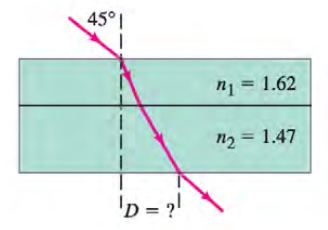
\includegraphics[width=0.3\textwidth]{figures/p43.jpg}
    \end{center}
\end{figure}
\begin{align*}
    \intertext{Snell's Law: $n_1\sin\theta_1 = n_2\sin\theta_2$, multiple
    iterations needed}
    \intertext{air($n_1$) $\Rightarrow$ $n_2=1.62$}
    \theta_2 &= \sin^{-1}\bp{\displaystyle\frac{n_1}{n_2}\sin\theta_1} \\
    \theta_2 &= \sin^{-1}\bp{\displaystyle\frac{1}{1.62}\sin 45\degree } \\
    \theta_2 &\approx 25.87987\degree \\
    \intertext{$n_1=1.62$ $\Rightarrow$ $n_2=1.47$}
    \theta_2 &= \sin^{-1}\bp{\displaystyle\frac{1.62}{1.47}\sin 25.87987\degree} \\
    \theta &\approx 28.75237\degree 
\end{align*}
\intertext{Using trigonometric identities,}
\begin{gather*}
    \tan\theta = \displaystyle\frac{opp}{adj} \\
    \tan\theta_1 = \displaystyle\frac{D_1}{h_1} \qquad \tan\theta_2 = \displaystyle\frac{D_2}{h_2} \\
    D_1 = h_1\tan\theta_1 \qquad D_2 = h_2\tan\theta_2 \\
\end{gather*}
\intertext{If $D = D_1 + D_2$,}
\begin{align*}
    D &= h_1\tan\theta_1 + h_2\tan\theta_2 \\
    D &= (2.0\;cm)\tan 25.87987\degree + (3.0\;cm)\tan 28.75237\degree \\
    \Aboxed{D &\approx 2.6\;cm}
\end{align*}
\newpage
\subsubsection*{
    44. An aquarium filled with water has flat glass sides whose index of refraction
    is 1.56. A beam of light from outside the aquarium strikes the glass at a 43.5°
    angle to the perpendicular. What is the angle of this light ray when it enters
    (a) the glass, and then (b) the water? (c) What would be the refracted angle
    if the ray entered the water directly?
}
\begin{figure}[h]
    \begin{center}
        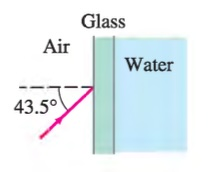
\includegraphics[width=0.3\textwidth]{figures/p44.jpg}
    \end{center}
\end{figure}
\begin{align*}
    \intertext{(a) air($n_1$) $\Rightarrow$ glass($n_2$)}
    \theta_2 &= \sin^{-1}\bp{\displaystyle\frac{n_1}{n_2}\sin\theta_1} \\
    \theta_2 &= \sin^{-1}\bp{\displaystyle\frac{1.00}{1.56}\sin 43.5\degree} \\
    \Aboxed{\theta_2 &= 26.2\degree}
    \intertext{(b) glass($n_1$) $\Rightarrow$ water($n_2$)}
    \theta_2 &= \sin^{-1}\bp{\displaystyle\frac{n_1}{n_2}\sin\theta_1} \\
    \theta_2 &= \sin^{-1}\bp{\displaystyle\frac{1.56}{1.33}\sin 26.2\degree} \\
    \Aboxed{\theta_2 &= 31.2\degree}
    \intertext{(c) air($n_1$) $\Rightarrow$ water($n_2$)}
    \theta_2 &= \sin^{-1}\bp{\displaystyle\frac{n_1}{n_2}\sin\theta_1} \\
    \theta_2 &= \sin^{-1}\bp{\displaystyle\frac{1.00}{1.33}\sin 43.5\degree} \\
    \Aboxed{\theta_2 &= 31.2\degree}
\end{align*}
\newpage 
\begin{center}
    \subsection*{\textbf{\textit{32-6 Visible Spectrum; Dispersion}}}
\end{center}
\subsubsection*{
    52. By what percent is the speed of blue light (450 nm) less than the speed of
    red light (680 nm), in silicate flint glass
} 
\begin{figure}[h]
    \begin{center}
        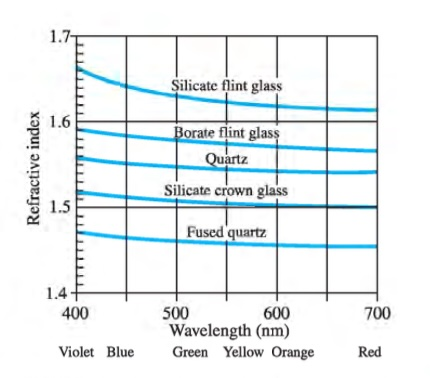
\includegraphics[width=0.3\textwidth]{figures/p52.jpg}
    \end{center}
\end{figure}
\begin{align*}
    \displaystyle\frac{v_{red}-v_{blue}}{v_{red}} &=
    \displaystyle\frac{\displaystyle\frac c
    {n_{red}}-\displaystyle\frac c {n_{blue}}}{\displaystyle\frac c {n_{red}}} =
    \displaystyle\frac{\displaystyle\frac{1}{1.613}-\displaystyle\frac{1}{1.643}}{\displaystyle\frac{1}{1.613}} \\
    \Aboxed{&\approx 0.01826 \approx 1.8\%}
\end{align*}
\spc
\begin{center}
    \subsection*{\textbf{\textit{32-7 Total Internal Reflection}}}
\end{center}
\subsubsection*{
    57. What is the critical angle for the interface between water and diamond?
    To be internally reflected, the light must start in which material?
}
\begin{align*}
    \intertext{$\theta_c$ is given by $\sin\theta_c = \displaystyle\frac {n_2}{n_1}\sin
    90\degree = \displaystyle\frac {n_2}{n_1}$}
    \intertext{water($n_1$) $\Rightarrow$ diamond($n_2$)}
    \theta_c &= \sin{-1}\bp{\displaystyle\frac{n_2}{n_1}} \\
    \theta_c &= \sin{-1}\bp{\displaystyle\frac{2.42}{1.33}} \\
    \intertext{Error at this angle which means there is total internal
    reflection}
    \intertext{diamond($n_1$) $\Rightarrow$ water($n_2$)}
    \theta_c &= \sin{-1}\bp{\displaystyle\frac{n_2}{n_1}} \\
    \theta_c &= \sin{-1}\bp{\displaystyle\frac{1.33}{2.42}} \\
    \theta_c &= 33.3\degree \\
    \Aboxed{\therefore &\text{To be internally reflected, the light must start
    with diamond}}
\end{align*}
\subsubsection*{
    58. The critical angle for a certain liquid-air surface is 49.6°. What is the
    index of refraction of the liquid?
}
\begin{gather*}
    \intertext{liquid($n_1$) $\Rightarrow$ air($n_2$)}
    \sin 49.6\degree = \displaystyle\frac{n_2}{n_1} \\
    n_1 = \displaystyle\frac{1.00}{\sin 49.6\degree} \\
\end{gather*}
\centerline{\Aboxed{n_1 \approx 1.31}}
\subsubsection*{
    61. A beam of light is emitted 8.0 cm beneath the surface of a liquid and strikes
    the surface 7.6 cm from the point directly above the source. If total internal
    reflection occurs, what can you say about the index of refraction of the liquid?
}
\begin{gather*}
    \tan\theta_1 = \displaystyle\frac{7.6\;cm}{8.0\;cm} \\
    \text{Incident Angle} = \theta_1 = \tan^{-1}\bp{\displaystyle\frac{7.6\;cm}{8.0\;cm}} \\
    \theta_1 \approx 43.5\degree \\
    \intertext{Relationship for the max incident angle for refraction from
    liquid into air} 
    n_1\sin\theta_{max} = n_2\sin 90\degree \\
    n_1\sin\theta_{max} = n_2 \\
    \intertext{So,}
    \sin\theta_1 \geq \sin\theta_{max} = \displaystyle\frac{1.00}{n_{liquid}} \\
    \sin\theta_1 \geq \displaystyle\frac{1.00}{n_{liquid}} \\
    0.688355 \geq \displaystyle\frac{1.00}{n_{liquid}}
\end{gather*}
\centerline{\Aboxed{\therefore n_{liquid} \geq 1.5}}
\end{document}
